\chapter{BurnDown Chart}
\label{sec:burndown-chart}
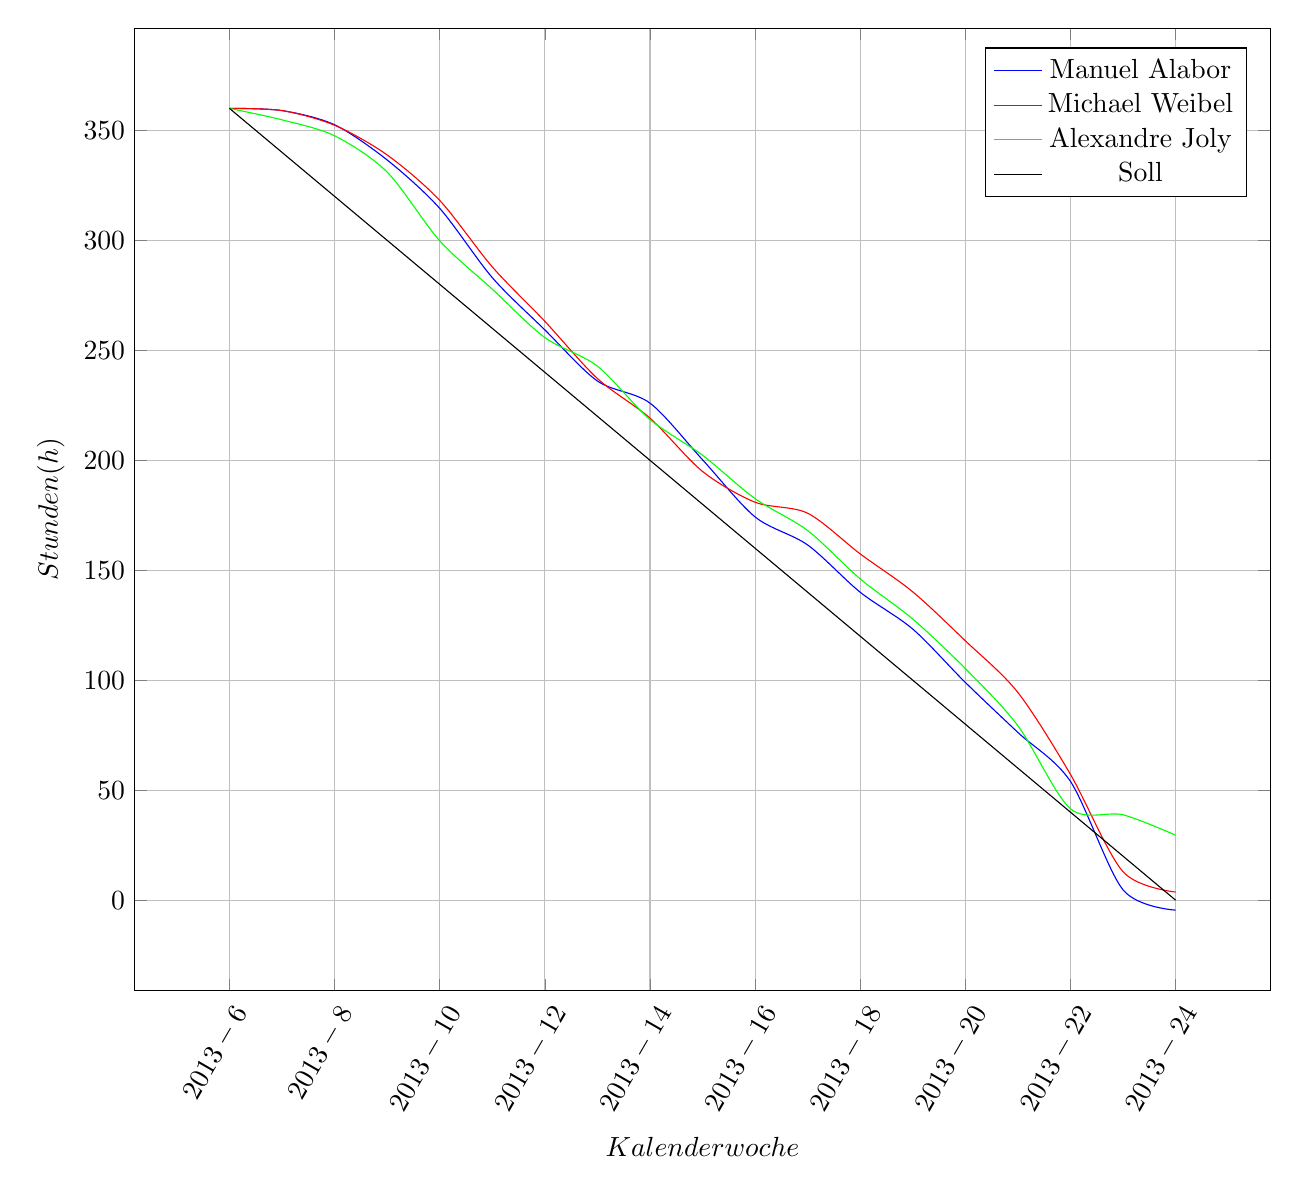
\begin{tikzpicture}
	\begin{axis}[
		width=16cm,
		xlabel=$Kalenderwoche$,
		ylabel=$Stunden (h)$,
		grid=major,
		xticklabels={
					$2013-2$,
					$2013-4$,
					$2013-6$,
					$2013-8$,
					$2013-10$,
					$2013-12$,
					$2013-14$,
					$2013-16$,
					$2013-18$,
					$2013-20$,
					$2013-22$,
					$2013-24$},
		every x tick label/.append style={
			xshift=-5pt,
			rotate=60
		}
	]
	\addplot[smooth,blue]
		plot coordinates {
			(6,360)
			(7,359)
			(8,352.55)
			(9,336.55)
			(10,314.55)
			(11,283.05)
			(12,259.3)
			(13,236.05)
			(14,226)
			(15,200.25)
			(16,174.25)
			(17,161.5)
			(18,140)
			(19,123.25)
			(20,99)
			(21,76.25)
			(22,54)
			(23,4.7)
			(24,-4.55)
		};
	\addlegendentry{Manuel Alabor}

	\addplot[smooth,color=red]
		plot coordinates {
			(6,360)
			(7,359)
			(8,352.33)
			(9,338.83)
			(10,318.17)
			(11,287.93)
			(12,263.18)
			(13,237.18)
			(14,219.18)
			(15,194.93)
			(16,180.93)
			(17,175.93)
			(18,157.43)
			(19,140.18)
			(20,117.93)
			(21,94.4299999999999)
			(22,57.1799999999999)
			(23,12.9299999999999)
			(24,3.67999999999995)
		};
	\addlegendentry{Michael Weibel}

	\addplot[smooth,color=green]
		plot coordinates {
			(6,360)
			(7,354.8)
			(8,347.55)
			(9,331.05)
			(10,299.8)
			(11,277.8)
			(12,255.8)
			(13,242.8)
			(14,218.55)
			(15,202.3)
			(16,182.55)
			(17,168.05)
			(18,146.05)
			(19,127.8)
			(20,105.3)
			(21,79.3)
			(22,41.55)
			(23,38.8)
			(24,29.55)
		};
	\addlegendentry{Alexandre Joly}

	\addplot[smooth,color=black]
		plot coordinates {
		(6,360)
		(7,340)
		(8,320)
		(9,300)
		(10,280)
		(11,260)
		(12,240)
		(13,220)
		(14,200)
		(15,180)
		(16,160)
		(17,140)
		(18,120)
		(19,100)
		(20,80)
		(21,60)
		(22,40)
		(23,20)
		(24,0)
		};
	\addlegendentry{Soll}
	\end{axis}
\end{tikzpicture}